\chapter{Implementation}\label{cap:implementacion}

\section{Introduction}
There are infinitely many ways of implementing sensors in a computer system. Internet of things is slowly becoming a topic that people interested in technology are talking about. For our particular case, we will be using an Arduino MEGA 2560 board

\section {How it works}

\section{Arduino}
Let's talk a bit more about the ingredients needed for the implementation of the sensors. We know we will be working with an Arduino MEGA 2560 board, but it goes withoutsaying, we will also need some more components. 

\subsection{FC-28 Soil Moisture Sensor}
Soil moisture sensor is likely the main sensor when harvesting is concerned as it helps farmers manage their irrigation systems more efficiently. This won't only save water but will also increase the quality of the crops since it can control moisture to the milimeter at all diferent plant growth stages. In this section, we are going to be documenting the process of using the sensor FC-28 with our Arduino board.

\subsubsection{How does it work?}
This FC-28 hygrometer module consists of two probes that measure the volumetric content of water. The current passes through the soil, which gives the resistance value between the metallic probes and measures the moisture value. The reason why this works fine is simple: the more water a soil has, the more electricity will be conducted which means less resistance.

\begin{figure}[htp]
    \centering
    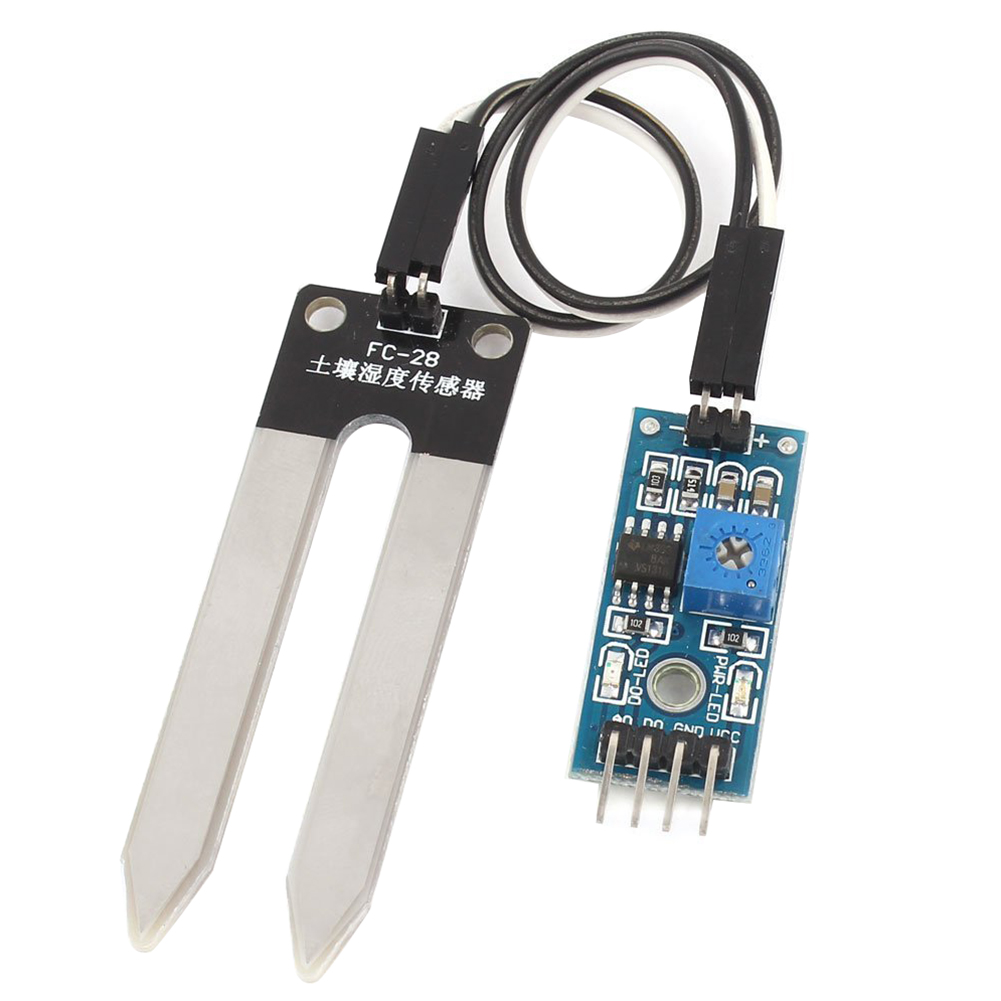
\includegraphics[width=0.35\textwidth]{fig/fc28.jpg}
    \caption{A FC-28 moisture sensor}
    \label{fig:fc28}
\end{figure}

Besides the sensor itself, there is another component that has two LEDs (one for output and another for power), a potentiometer and a LM293 comparator.

\subsubsection{Using the sensor}
The values that the sensor picks up goes from 0 to 1023. Ideally it would show 0 when sunken underwater and 1023 when is only in contact with the air, in other words, when it's not in contact with soil.

Let's implement a small script to understand the behaviour of the sensor. The circuit that we will be using is really simple:
\begin{itemize}
	\item The VCC of the FC-28 goes to 5V of the Arduino
	\item The GND of the FC-28 goes to GND of the Arduino
	\item The pin A0 of the FC-28 goes to the pin A0 of the Arduino
\end{itemize}
This circuit looks like this:
	\begin{figure}[htp]
		\centering
		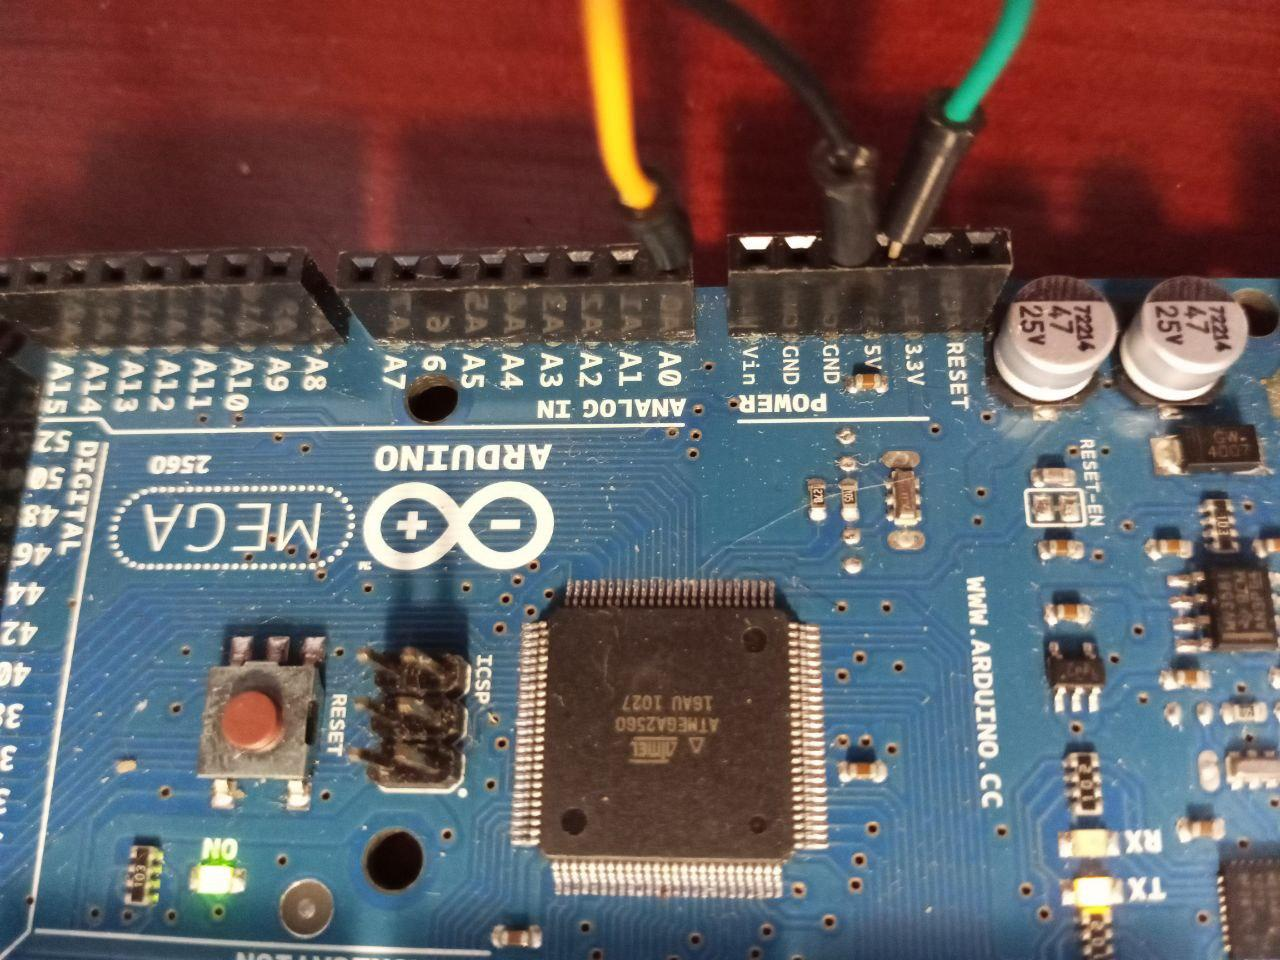
\includegraphics[width=0.35\textwidth]{fig/fc28-circuit1.jpg}
		\caption{fc28-circuit1}
	\end{figure}
	\hfill
	\begin{figure}[htp]
		\centering
		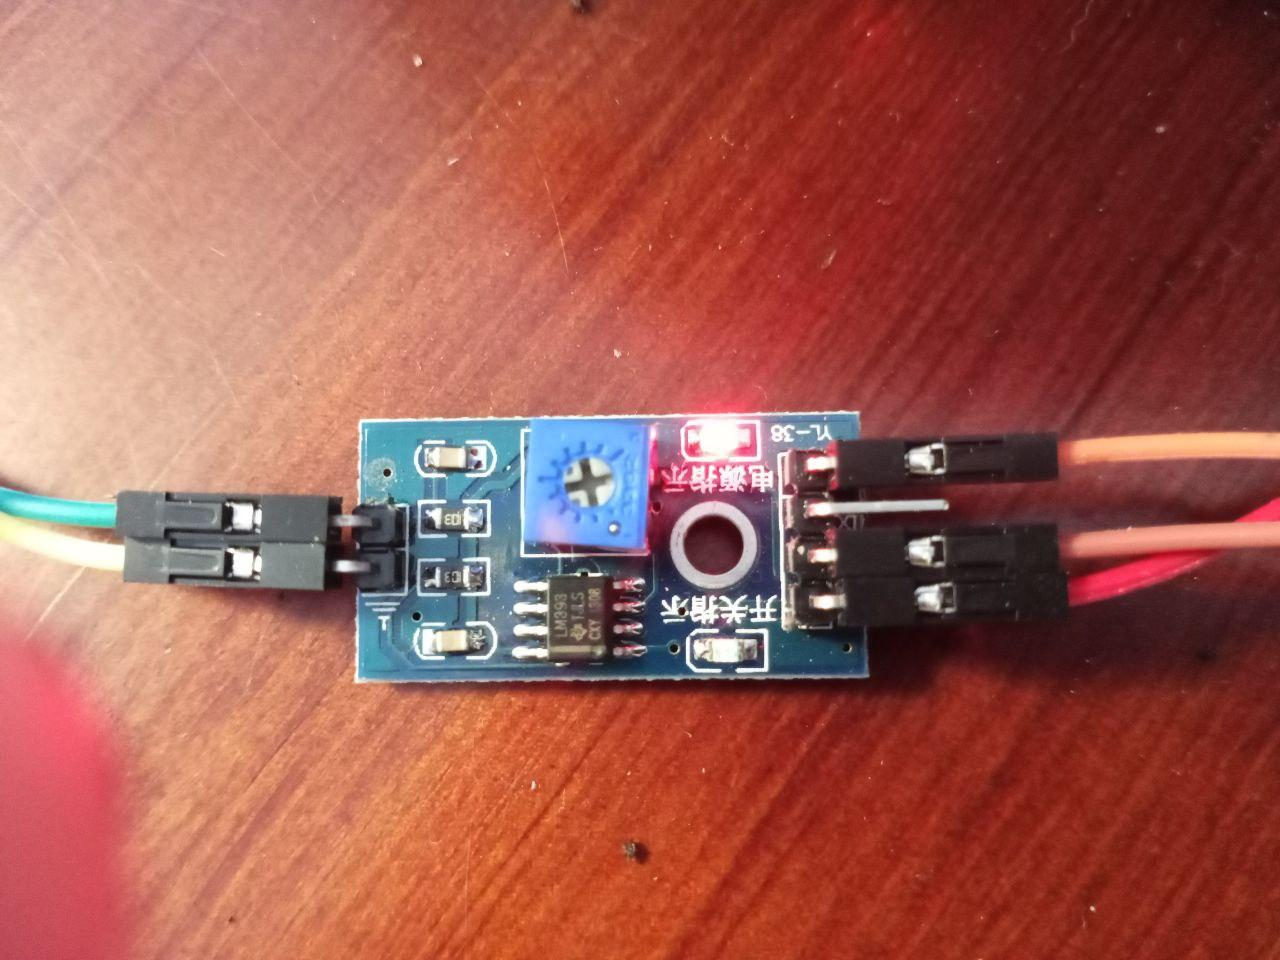
\includegraphics[width=0.35\textwidth]{fig/fc28-circuit2.jpg}
		\caption{fc28-circuit2}
	\end{figure}

Now let's take a look at the script that is going to make the sensor work

\lstinputlisting{arduino/fc28.ino}

\subsection{Photoresistor}

\section{Conclusions}


